\documentclass{article}
\usepackage[T1]{fontenc}
\usepackage{lmodern}
\usepackage{graphicx}
\usepackage{amsmath,amssymb}
\usepackage[a4paper,margin=2cm]{geometry}
\usepackage[absolute,overlay]{textpos}
\setlength{\TPHorizModule}{1mm}
\setlength{\TPVertModule}{1mm}
\usepackage[indonesian]{babel}
\usepackage{hyperref}
\setlength{\emergencystretch}{2em}
% unit: Halaman 42

\begin{document}

% === Halaman 42 (python/native) ===

The EFF's US\$250,000 DES cracking machine contained 1,856 

custom chips and could brute force a DES key in a matter of days 

— the photo shows a DES Cracker circuit board fitted with several 

Deep Crack chips (Sumber Wikipedia). 

42

% deskripsi: gambar native xref 190
\noindent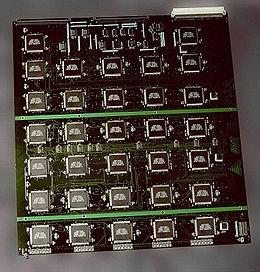
\includegraphics[width=0.85\textwidth]{../../images/python/page_042_img_01.jpeg}

\end{document}
